
% \section{The Architecture of NetAlly}


% \subsection{Multi-Agent Debate System}

% MAS is built on LangGraph that improves the reliability and reasoning accuracy of network QA.
% Five specialized agents share state across a two-phase pipeline: an information refinement phase (\textit{Phase~1}) and an adversarial verification phase (\textit{Phase~2}).
% This hierarchical design addresses the hallucination and context leakage problems that arise when a single LLM processes large network configuration files.

% \begin{figure}[!t]
%   \centering
%   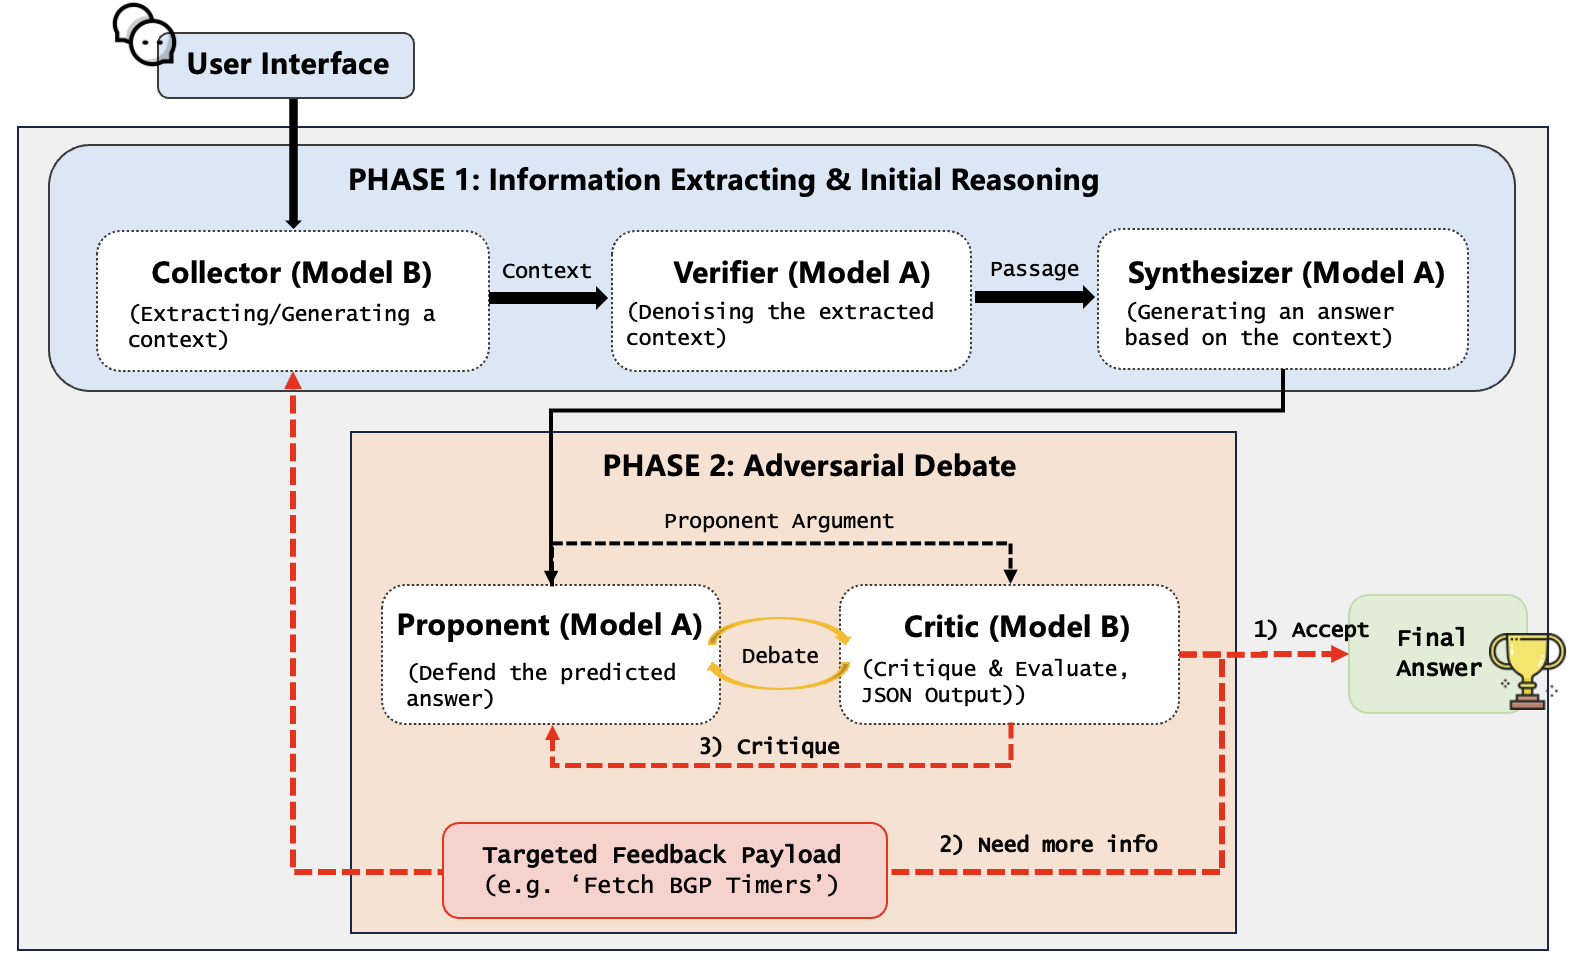
\includegraphics[width=1.05c\columnwidth]{figure/multi_agent_arch.png}
%   \caption{Multi-agent debate and hierarchical feedback architecture of NetAgent.}
%   \label{fig:multi_agent_arch}
% \end{figure}

% % ============================================================
% \subsection{Agent Roles}
% % ============================================================

% The MAS comprises collector, verifier, synthesizer, proponent and critic.
% The \textbf{Collector} extracts relevant configuration blocks from the raw context (or generates context from domain knowledge when none is available) and revises its extraction scope upon Outer Loop re-entry.
% The \textbf{Verifier} filters noise from the extracted context to produce a clean passage; for L4/L5 questions requiring full topology reasoning, filtering is bypassed (\textbf{BYPASS}).
% The \textbf{Synthesizer} derives a candidate answer from the passage; for L5 fault-analysis questions, it follows a six-step structured inference procedure.
% The \textbf{Proponent} constructs a passage-grounded supporting argument and, upon receiving critique, refines the candidate answer via \textit{Self-Refine}~\cite{madaan2023selfrefine}.
% The \textbf{Critic} renders one of three verdicts based on passage evidence:

% \begin{equation}
% \small
%   \text{verdict} =
%   \begin{cases}
%     \textit{ACCEPT}           & \text{if } \text{evidence}(p, a) = \text{True} \\
%     \textit{CONTINUE\_DEBATE} & \text{if } \text{evidence}(p, a) = \text{Partial} \\
%     \textit{NEED\_MORE\_INFO} & \text{if } \text{evidence}(p, a) = \text{None}
%   \end{cases}
% \end{equation}
% end{table}

% %============================================================
% \subsection{Hierarchical Loop Structure}
% % ============================================================

% The Critic's verdict drives a two-level feedback loop.
% An \textit{ACCEPT} verdict terminates the pipeline and outputs the consensus answer.
% A \textit{CONTINUE\_DEBATE} verdict triggers an \textbf{Inner Loop}: the Proponent refines the answer based on the critique and resubmits to the Critic (up to 3 turns).
% A \textit{NEED\_MORE\_INFO} verdict triggers an \textbf{Outer Loop}: the Collector re-extracts context guided by the feedback payload and restarts the pipeline (up to 3 iterations).
% This structure combines adversarial debate~\cite{du2024improving} and skeptical verification~\cite{liang2024encouraging} to substantially improve factual accuracy in the network configuration domain.




% \subsection{설계 동기: 왜 도메인 학습이 아닌 3-Plane 통합인가}
% L4/L5의 성능 격차를 해소하는 접근으로 도메인 특화 학습(fine-tuning)과 기존 분석 도구 통합이 있다. 우리는 후자를 채택하였다. 네트워크 설정 파일은 벤더와 OS 버전에 따라 구문이 상이하여 학습 데이터 확보가 어렵고, L4/L5 태스크는 그래프 알고리즘의 실행을 요구하므로 학습량을 늘려도 정확도 상한이 존재한다. 반면 Batfish와 같이 이미 검증된 분석 도구를 활용하면 정확도와 신뢰성을 동시에 확보할 수 있다.

% \begin{figure}[!t]
%   \centering
%   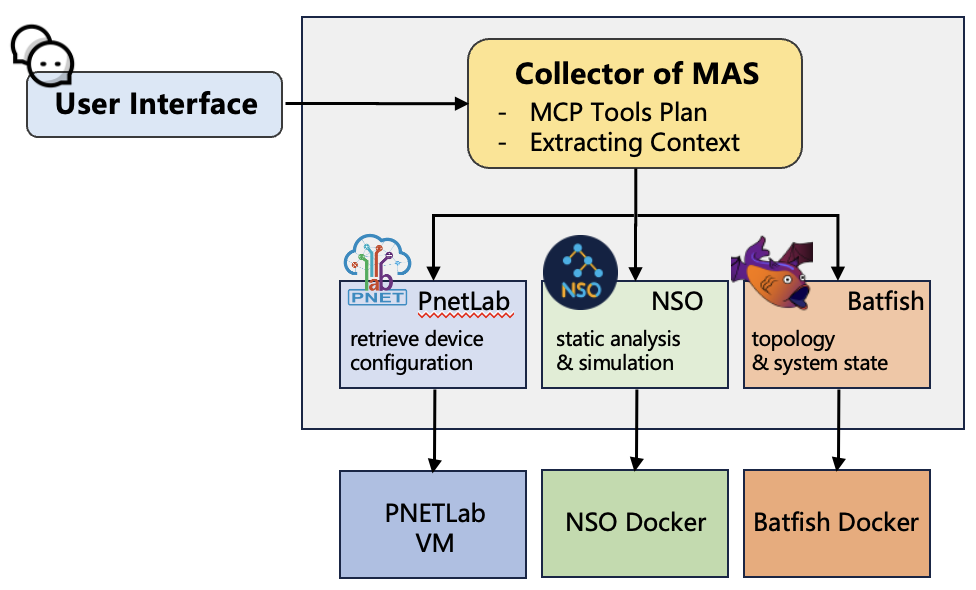
\includegraphics[width=0.4\textwidth]{figure/netally_arch.png}
%   \caption{NetAlly 3-Plane Architecture. The Orchestrator analyzes the query to select relevant skills, and the Executor invokes tools across the PNETLab, NSO, and Batfish planes through a ReAct loop.}
%   \label{fig:netally-arch}
% \end{figure}


% \subsection{3-Plane 통합 아키텍처}
% Fig.~\ref{fig:netally-arch}에 나타낸 바와 같이, NetAlly는 세 개의 독립된 네트워크 관리 평면을 하나의 Chat 인터페이스로 통합한다: (1) \textbf{PNETLab Plane} --- 가상 토폴로지 관리, 장비 부팅, 콘솔 접근, (2) \textbf{NSO Plane} --- RESTCONF 기반 구성 조회\textperiodcentered 동기화\textperiodcentered 변경, (3) \textbf{Batfish Plane} --- 정형 검증, traceroute 시뮬레이션, What-If 분석. 이 세 평면의 도구들은 MCP를 통해 에이전트에 노출되며, Orchestrator--Executor 구조가 LangGraph~\cite{ref3} 기반 상태 기계(State Machine) 위에서 질의의 성격에 따라 적절한 평면의 도구를 선택한다.

% \textbf{Orchestrator (계획 에이전트):} 경량 LLM이 스킬 카탈로그(각 스킬의 이름, 설명, 필요 도구가 YAML 프론트매터로 정의된 SKILL.md 파일 집합)와 사용자 질의를 입력받아, JSON 형식으로 1-3개의 관련 스킬을 선택하고 선택 근거를 출력한다. 예를 들어, ``P1-P2 링크 장애 시 PE1$\rightarrow$Leaf3 경로는?''이라는 질의에 대해 Orchestrator는 \texttt{["core", "network\_verify"]}를 선택하고, ``What-If 분석이 필요하므로 Batfish fork\_snapshot을 사용해야 한다''는 추론을 생성한다. 선택된 스킬의 상세 가이드(SKILL.md 본문)가 Executor의 시스템 프롬프트에 주입되어, 도구 호출의 맥락과 제약 조건을 전달한다.

% \textbf{Executor (실행 에이전트):} Executor LLM은 Orchestrator가 주입한 스킬 프롬프트와 16개 이상의 MCP 도구 바인딩을 기반으로 ReAct(Reason-Act-Observe) 루프를 수행한다. 각 반복에서 대화 이력을 분석하여 다음 행동을 결정하고, 도구를 호출한 뒤 출력을 관찰하여 추가 호출 여부를 판단한다. 최종 답변이 도출되거나 최대 10단계에 도달하면 루프가 종료된다.


% \subsection{다층 오류 복구 메커니즘}
% NetAlly는 다층 오류 복구(Multi-layer Error Recovery)를 통해 단순 도구 래퍼(Wrapper)와 차별화된다. 도구 호출 실패를 Python 예외로 전파하지 않고, 구조화된 오류 딕셔너리(\texttt{\{"error": ..., "tool": ...\}})로 변환하여 LLM의 대화 이력에 삽입한다. 이를 통해 LLM은 다음 반복에서 (a)~다른 도구로 전환, (b)~동일 도구를 수정된 파라미터로 재호출, (c)~부분적 결과로 최선의 답변 생성 중 하나를 선택한다. 이 외에도 \texttt{async} 호출 실패 시 \texttt{sync} 스레드로의 자동 폴백, \texttt{NETALLY\_MCP\_ALLOW\_MUTATIONS} 플래그를 통한 읽기 전용 모드 강제, 10회 반복 후 강제 종료를 통한 무한 루프 방지, 미포착 예외의 SSE \texttt{error} 이벤트 변환 등의 안전 장치를 포함한다. 예를 들어, Batfish가 특정 설정 파일을 파싱하지 못하는 경우에도 에이전트는 NSO 쿼리로 대안을 시도하며, 완전한 실패보다 부분적 답변을 우선한다.

% \subsection{핵심 도구와 자율 파이프라인}
% Executor가 호출하는 핵심 도구는 세 가지이다: (1)~\texttt{network\_query}는 Cisco NSO RESTCONF를 통해 실시간 구성을 조회하며 L1- L3에 주로 활용된다. (2)~\texttt{network\_verify}는 Batfish를 통해 정형 검증과 What-If 분석을 수행하며 L4- L5에 활용된다. (3)~\texttt{lab\_manage}는 PNETLab 토폴로지 관리 및 자동 온보딩을 담당한다.
% NetAlly는 두 가지 자동화 파이프라인을 통해 수동 조작을 최소화한다.

% \textbf{자율 온보딩.} Section~V의 실험에서 4개 Lab의 설정 파일 수집과 Batfish 스냅샷 초기화에 사용된다. PNETLab의 가상 장비를 사람의 CLI 조작 없이 운영 가능 상태로 전환한다. 파이프라인은 (1)~LabFS에서 토폴로지와 콘솔 포트를 파싱하고, (2)~각 장비에 Telnet으로 접속하여 SSH를 활성화하며, (3)~NSO에 RESTCONF로 등록 후 설정을 동기화하고, (4)~수집된 설정으로 Batfish 스냅샷을 초기화한다. IOS 버전별 명령어 호환성, 관리 IP 충돌, 동기화 실패 시 자동 재시도 등의 예외 처리가 포함된다.

% \textbf{Fork-Snapshot 기반 What-If 분석.} L5 장애 영향 추론을 지원하기 위해, Batfish의 \texttt{fork\_snapshot}으로 지정된 변경(링크/노드 비활성화)을 적용한 가상 네트워크 복사본을 생성한다. 원본 스냅샷은 보존되므로 비파괴적이다. 생성된 복사본에 \texttt{differentialReachability} 쿼리를 실행하여, 장애 전후의 도달성 차이를 식별하고 영향 범위를 도출한다. 이 과정은 에이전트가 수행하며, 운영자는 ``P1-P2 링크가 다운되면 어떤 영향이 있는가?''와 같은 자연어 질의만 제공하면 된다.



\section{The Architecture of NetAlly}

% ============================================================
\subsection{시스템 개요}
% ============================================================

NetAlly는 MCP 기반 도구 호출과 Multi-Agent Debate를 결합한
네트워크 설정 분석 시스템이다.
단일 LLM이 설정 파일을 정적으로 처리하는 기존 방식과 달리,
NetAlly는 5개의 전문화된 에이전트가 역할을 분담하여 질의를 처리하고,
각 에이전트가 필요에 따라 NSO 및 Batfish 도구를 자율적으로 호출한다.
Fig.~\ref{fig:netally-arch}에 나타낸 바와 같이,
세 개의 독립된 네트워크 관리 평면이 단일 인터페이스로 통합된다:
(1)~\textbf{PNETLab Plane} --- 가상 토폴로지 관리 및 장비 접근,
(2)~\textbf{NSO Plane} --- RESTCONF 기반 실시간 구성 조회,
(3)~\textbf{Batfish Plane} --- 정형 검증, traceroute 시뮬레이션, What-If 분석.
이 세 평면의 도구들은 MCP를 통해 에이전트에 노출되며, Collector 에이전트가 질의 유형에 따라 적절한 도구를 선택하여 호출한다. 


\begin{figure}[!t]
  \centering
  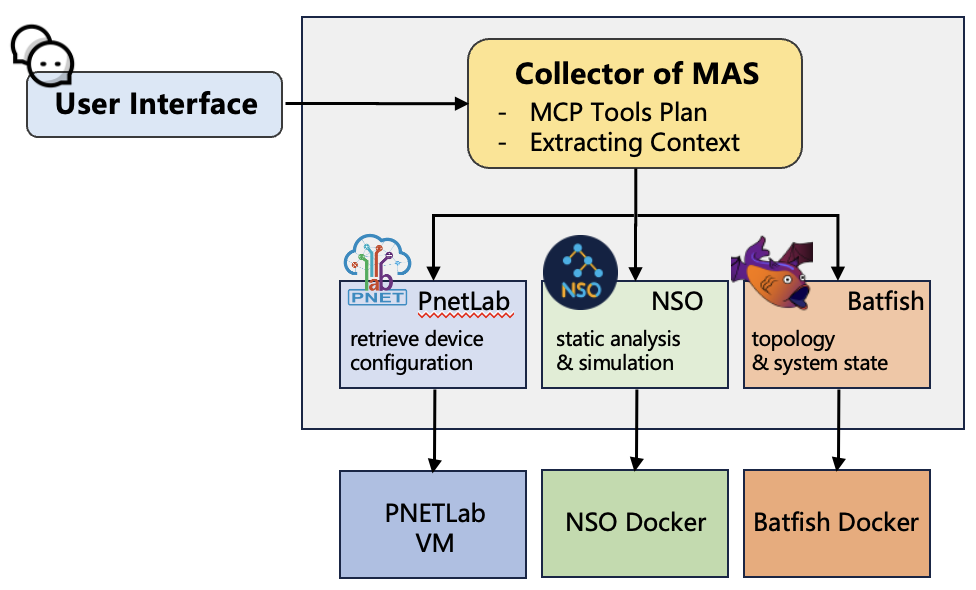
\includegraphics[width=0.45\textwidth]{figure/netally_arch.png}
  \caption{NetAlly 3-Plane Architecture. The Collector selects and invokes tools across the NSO and Batfish planes via MCP,
  and the debate pipeline ensures answer reliability.}
  \label{fig:netally-arch}
\end{figure}

% ============================================================
% \subsection{설계 동기: 왜 도메인 학습이 아닌 도구 통합인가}
% % ============================================================

% L4/L5의 성능 격차를 해소하는 접근으로 도메인 특화 학습(fine-tuning)과
% 기존 분석 도구 통합이 있다. 우리는 후자를 채택하였다.
% 네트워크 설정 파일은 벤더와 OS 버전에 따라 구문이 상이하여
% 학습 데이터 확보가 어렵고,
% L4/L5 태스크는 그래프 알고리즘의 실행을 요구하므로
% 학습량을 늘려도 정확도 상한이 존재한다.
% 반면 Batfish와 같이 이미 검증된 분석 도구를 활용하면
% 정확도와 신뢰성을 동시에 확보할 수 있다.

% ============================================================
\subsection{Multi-Agent Debate System}
% ============================================================

NetAlly의 답변 생성 파이프라인은 LangGraph~\cite{ref3} 기반
5-Agent 토론 구조 위에 구현된다.
파이프라인은 정보 정제 단계(\textit{Phase~1})와
적대적 검증 단계(\textit{Phase~2})로 구성되며,
단일 LLM이 대용량 설정 파일을 처리할 때 발생하는
환각(hallucination) 및 컨텍스트 누수 문제를 해소한다.
agents\_v3(Pure MAS)와 동일한 5-Agent 구조를 유지하되,
Collector에 MCP 도구 선택 및 호출 능력을 추가한 것이
NetAlly의 핵심 확장이다.

\begin{figure}[!t]
  \centering
  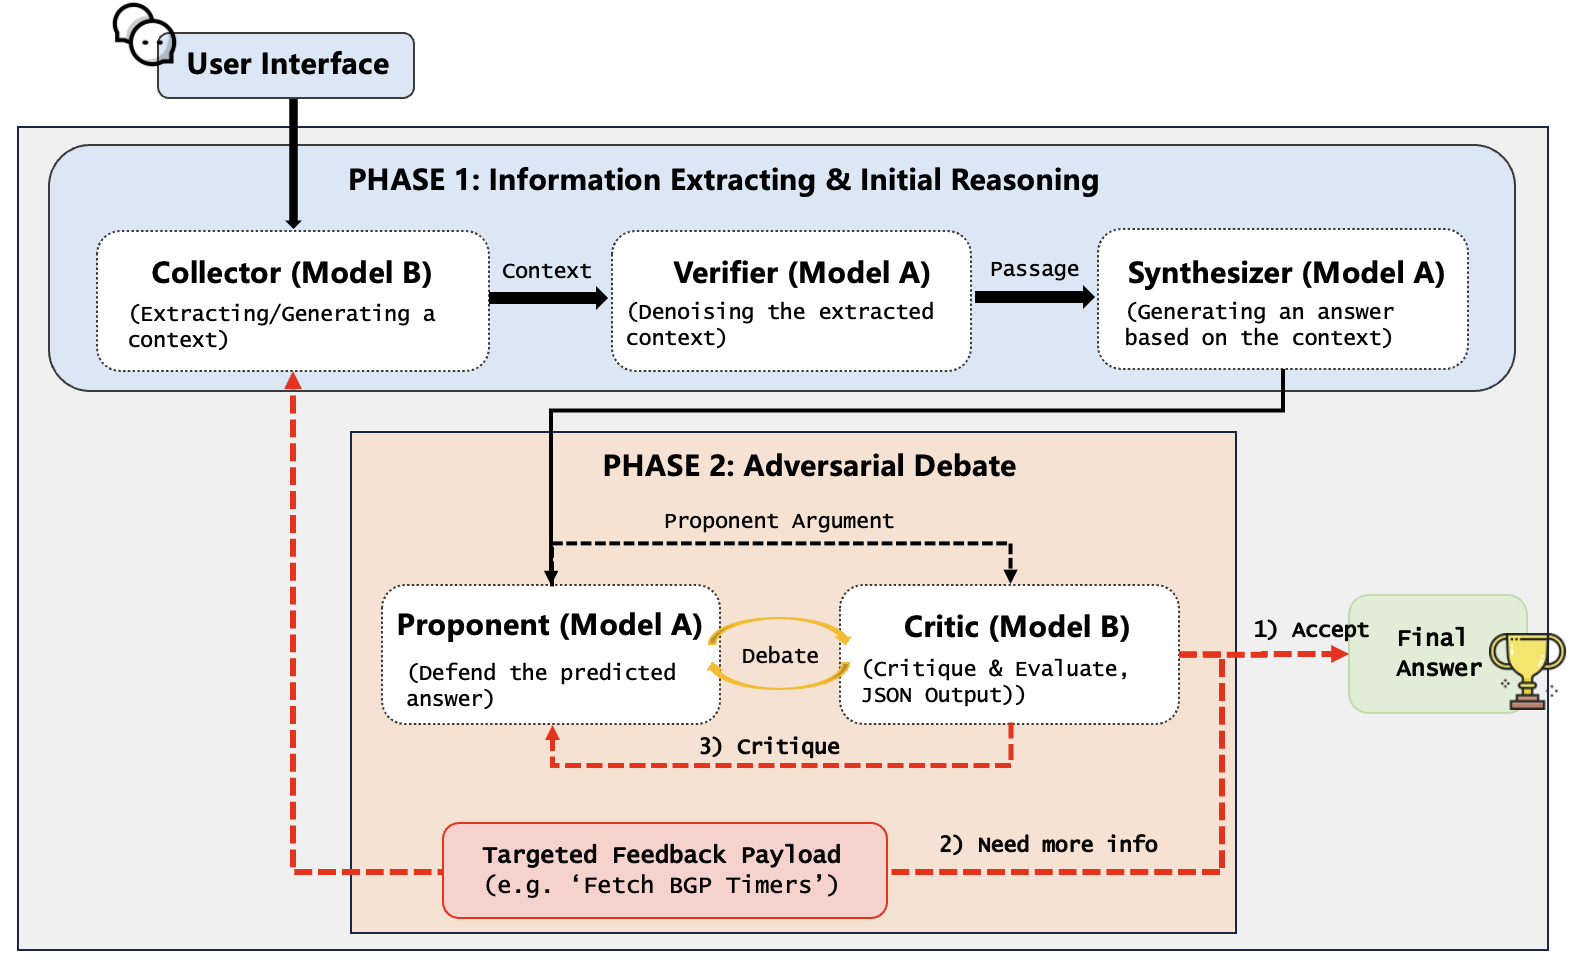
\includegraphics[width=1.05\columnwidth]{figure/multi_agent_arch.png}
  \caption{Multi-agent debate and hierarchical feedback architecture
  of NetAlly. The Collector selects MCP tools based on question level
  and feeds structured tool results into the debate pipeline.}
  \label{fig:multi_agent_arch}
\end{figure}

% ============================================================
\subsubsection{Agent 역할}
% ============================================================

MAS는 Collector, Verifier, Synthesizer, Proponent, Critic으로 구성된다.

\textbf{Collector}는 질의와 레벨(L1--L5)을 분석하여
도구 카탈로그에서 적절한 MCP 도구를 선택하고
JSON 형식의 도구 호출 계획을 생성한 뒤 순차적으로 실행한다.
도구 선택 기준은 질의 레벨에 따라 결정된다:
L1은 \texttt{nso\_get\_device\_info()} 단일 호출, L2는 캐시된 \texttt{nso\_get\_all\_device\_info()}, L3는 \texttt{nso\_get\_all\_*} 및 \texttt{batfish\_bgp\_sessions()}, L4는 \texttt{batfish\_traceroute()} 또는 \texttt{batfish\_reachability()}, L5는 \texttt{nso\_get\_all\_device\_info()}로 토폴로지를 파악한 후 \texttt{batfish\_*\_failure()} 계열 도구로 장애를 시뮬레이션한다. Outer Loop 재진입 시에는 Critic의 피드백에 따라 추가 도구를 호출한다.

% \begin{itemize}
%   \item L1: \texttt{nso\_get\_device\_info()} 단일 호출
%   \item L2: 캐시된 \texttt{nso\_get\_all\_device\_info()}
%   \item L3: \texttt{nso\_get\_all\_*} 및 \texttt{batfish\_bgp\_sessions()}
%   \item L4: \texttt{batfish\_traceroute()} or \texttt{batfish\_reachability()}
%   \item L5: \texttt{nso\_get\_all\_device\_info()} 후 \texttt{batfish\_*\_failure()} 2단계 호출
% \end{itemize}

\textbf{Verifier}는 수집된 컨텍스트에서 노이즈를 제거하여
정제된 passage를 생성한다.
단, MCP 도구 결과가 포함된 경우 필터링을 우회(\textbf{BYPASS})하여
도구 출력을 권위 있는 증거(authoritative evidence)로 직접 처리한다.

\textbf{Synthesizer}는 passage로부터 후보 답변을 도출하며,
answer\_type별 포맷 힌트를 적용한다:
\texttt{set} 타입은 JSON 배열, \texttt{map} 타입은 JSON 객체,
\texttt{path} 타입은 \texttt{PE1 -> P2 -> PE2} 형식으로 출력한다.
L5 장애 분석 질의에 대해서는 6단계 구조적 추론 절차를 따른다.

\textbf{Proponent}는 passage에 근거한 지지 논거를 구성하고,
Critic으로부터 비판을 수신하면
\textit{Self-Refine}~\cite{madaan2023selfrefine}을 통해
후보 답변을 개선한다.

\textbf{Critic}은 passage 증거에 기반하여
다음 세 가지 판정 중 하나를 내린다:

\vspace{-8pt}
\begin{equation}
\footnotesize
  \text{verdict} =
  \begin{cases}
    \textit{ACCEPT}           & \text{if } \text{evidence}(p, a) = \text{True} \\
    \textit{CONTINUE\_DEBATE} & \text{if } \text{evidence}(p, a) = \text{Partial} \\
    \textit{NEED\_MORE\_INFO} & \text{if } \text{evidence}(p, a) = \text{None}
  \end{cases}
\end{equation}

MCP 도구 출력이 존재하는 경우,
Critic은 해당 출력을 권위 있는 증거로 간주하여
우선적으로 \textit{ACCEPT} 판정을 내린다.

% ============================================================
\subsubsection{계층적 루프 구조}
% ============================================================

Critic의 판정은 2단계 피드백 루프를 구동한다.
\textit{ACCEPT} 판정은 파이프라인을 종료하고 합의된 답변을 출력한다.
\textit{CONTINUE\_DEBATE} 판정은 \textbf{Inner Loop}를 트리거하며,
Proponent가 비판에 기반하여 답변을 개선하고
Critic에 재제출한다(최대 2회).
\textit{NEED\_MORE\_INFO} 판정은 \textbf{Outer Loop}를 트리거하며,
Collector가 피드백 페이로드에 따라 추가 MCP 도구를 호출하고
파이프라인을 재시작한다(최대 2회).
이 구조는 적대적 토론~\cite{du2024improving}과
회의적 검증~\cite{liang2024encouraging}을 결합하여
네트워크 설정 도메인에서의 사실 정확도를 크게 향상시킨다.

% ============================================================
\subsection{MCP 도구 통합}
% ============================================================

NetAlly는 총 18개의 MCP 도구를 제공하며,
Table~\ref{tab:mcp_tools}에 전체 목록을 정리하였다.
도구는 세 그룹으로 구분된다:
NSO RESTCONF 기반 도구 5개(L1--L3),
Batfish 정적 분석 도구 8개(L3--L4),
Batfish What-If 시뮬레이션 도구 5개(L5).

\textbf{도구 실행 엔진.}
Collector LLM이 질의와 레벨을 분석하여 JSON 형식의 도구 호출 계획을 생성하면,
\texttt{tool\_dispatch.py}가 이를 수신하여
\texttt{ThreadPoolExecutor}로 순차 실행하고
결과를 하위 에이전트가 소비할 수 있는 구조화된 텍스트로 변환한다.
도구 선택 기준은 질의 레벨에 따라 결정된다:
L1은 \texttt{nso\_get\_device\_info()} 단일 호출,
L2는 캐시된 \texttt{nso\_get\_all\_device\_info()},
L3는 \texttt{nso\_get\_all\_*} 및 \texttt{batfish\_bgp\_sessions()},
L4는 \texttt{batfish\_traceroute()} 또는 \texttt{batfish\_reachability()},
L5는 토폴로지 파악 후 \texttt{batfish\_*\_failure()} 계열로
장애를 시뮬레이션하는 2단계 호출을 수행한다.

\textbf{오류 복구.}
도구 호출 실패 시 Python 예외를 전파하지 않고,
구조화된 오류 딕셔너리(\texttt{\{"error":~...,~"tool":~...\}})를
LLM 대화 이력에 삽입한다.
이를 통해 에이전트는 다음 반복에서
(a)~다른 도구로 전환,
(b)~수정된 파라미터로 재호출,
(c)~부분적 결과로 최선의 답변 생성
중 하나를 자율적으로 선택한다.
예를 들어, Batfish가 특정 설정 파일을 파싱하지 못하는 경우
에이전트는 NSO 쿼리로 대안을 시도하며,
완전한 실패보다 부분적 답변을 우선한다.

\textbf{세션 캐싱 및 집계.}
\texttt{nso\_get\_all\_device\_info()} 및
\texttt{nso\_get\_all\_interfaces()}는 세션 내 캐싱을 적용하여
첫 호출 이후 추가 HTTP 요청 없이 즉시 결과를 반환한다.
또한 NSO 도구는 장비별 집계 결과를
\texttt{aggregations} 필드로 미리 계산하여 제공함으로써,
LLM이 개별 장비를 순회하며 필터링하는 부담을 제거한다.
예를 들어, ``AAA가 활성화된 장비는?''와 같은 L2 질의에 대해
LLM은 20개 장비의 config를 직접 파싱하는 대신
\texttt{aggregations.devices\_with\_aaa} 필드를 즉시 참조한다.

\begin{table}[!t]
\caption{MCP Tool Catalog of NetAlly (총 18개)}
\label{tab:mcp_tools}
\centering
\resizebox{\columnwidth}{!}{%
\begin{tabular}{clll}
\hline
\textbf{평면} & \textbf{도구명} & \textbf{기능} & \textbf{레벨} \\
\hline
\multirow{5}{*}{\shortstack{NSO\\RESTCONF}}
  & \texttt{nso\_get\_device\_info}      & 단일 장비 config 요약     & L1--L2 \\
  & \texttt{nso\_get\_all\_device\_info} & 전체 장비 + aggregations  & L2     \\
  & \texttt{nso\_get\_interfaces}        & 단일 장비 인터페이스 조회 & L1     \\
  & \texttt{nso\_get\_all\_interfaces}   & 전체 인터페이스 벌크 조회 & L2     \\
  & \texttt{nso\_get\_routing}           & BGP/OSPF 라우팅 조회      & L2--L3 \\
\hline
\multirow{4}{*}{\shortstack{Batfish\\Basic}}
  & \texttt{batfish\_traceroute}         & 경로 추적                 & L4     \\
  & \texttt{batfish\_reachability}       & 도달성 검사               & L4     \\
  & \texttt{batfish\_bgp\_sessions}      & BGP 세션 상태 분석        & L3--L4 \\
  & \texttt{batfish\_route\_table}       & 라우팅 테이블 조회        & L3--L4 \\
\hline
\multirow{4}{*}{\shortstack{Batfish\\(L4)}}
  & \texttt{batfish\_acl\_check}         & ACL 차단 분석             & L4     \\
  & \texttt{batfish\_loop\_check}        & 라우팅 루프 탐지          & L4     \\
  & \texttt{batfish\_blackhole\_check}   & 블랙홀 경로 탐지          & L4     \\
  & \texttt{batfish\_waypoint\_check}    & 경유 장비 검증            & L4     \\
\hline
\multirow{5}{*}{\shortstack{Batfish\\(L5 What-If)}}
  & \texttt{batfish\_link\_failure}        & 단일 링크 장애 시뮬레이션   & L5 \\
  & \texttt{batfish\_multi\_link\_failure} & 2-링크 동시 장애 시뮬레이션 & L5 \\
  & \texttt{batfish\_node\_failure}        & 단일 노드 장애 분석         & L5 \\
  & \texttt{batfish\_multi\_node\_failure} & 2-노드 동시 장애 분석       & L5 \\
  & \texttt{batfish\_spof\_detection}      & 단일 장애점(SPOF) 탐지      & L5 \\
\hline
\end{tabular}%
}
\end{table}

% ============================================================
\subsection{자율 파이프라인}
% ============================================================

NetAlly는 두 가지 자동화 파이프라인을 통해 수동 조작을 최소화한다.

\textbf{자율 온보딩.}
4개 Lab의 설정 파일 수집과 Batfish 스냅샷 초기화에 사용되며,
PNETLab의 가상 장비를 CLI 조작 없이 운영 가능 상태로 전환한다.
파이프라인은 (1)~LabFS에서 토폴로지와 콘솔 포트를 파싱하고,
(2)~각 장비에 Telnet으로 접속하여 SSH를 활성화하며,
(3)~NSO에 RESTCONF로 등록 후 설정을 동기화하고,
(4)~수집된 설정으로 Batfish 스냅샷을 초기화한다.
IOS 버전별 명령어 호환성, 관리 IP 충돌,
동기화 실패 시 자동 재시도 등의 예외 처리가 포함된다.

\textbf{Fork-Snapshot 기반 What-If 분석.}
L5 장애 영향 추론을 지원하기 위해,
Batfish의 \texttt{fork\_snapshot}으로 지정된 변경
(링크/노드 비활성화)을 적용한 가상 네트워크 복사본을 생성한다.
원본 스냅샷은 보존되므로 비파괴적이다.
생성된 복사본에 \texttt{differentialReachability} 쿼리를 실행하여
장애 전후의 도달성 차이를 식별하고 영향 범위를 도출한다.
운영자는 ``P1-P2 링크가 다운되면 어떤 영향이 있는가?''와 같은
자연어 질의만 제공하면 된다.